\section{Tree-To-Text Transformation with SDMs}
\begin{enumerate}
\item[$\blacktriangleright$] DictionaryTreeGrammar
  (Fig.~\ref{fig:moca-DictionaryTreeGrammar})    
  %\usepackage{graphics} is needed for \includegraphics
\begin{figure}[!htbp]
\begin{center}
 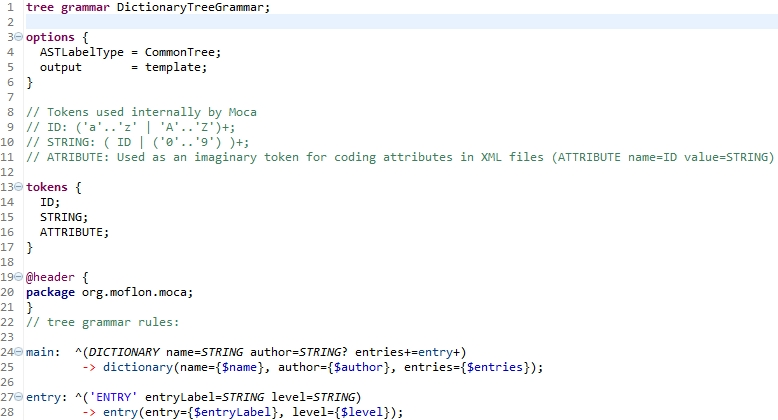
\includegraphics[width=\textwidth]{pics/moca/5MocaTreeToText/DictionaryTreeGrammar}
  \caption{Tree Grammar for the dictionary DSL} 
  \label{fig:moca-DictionaryTreeGrammar}
\end{center}
\end{figure} 

\item[$\blacktriangleright$] DictionaryUnparserAdapter
  (Fig.~\ref{fig:moca-DictionaryUnparserAdapter})    
  %\usepackage{graphics} is needed for \includegraphics
  
\begin{figure}[!htbp]
\begin{center}
 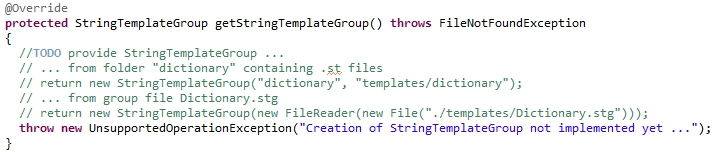
\includegraphics[width=\textwidth]{pics/moca/5MocaTreeToText/UnparserAdapterNotImplemented}
  \caption{Unimplemented method getStringTemplateGroup} 
  \label{fig:moca-DictionaryUnparserAdapter}
\end{center}
\end{figure} 
 
\begin{figure}[!htbp]
\begin{center}
 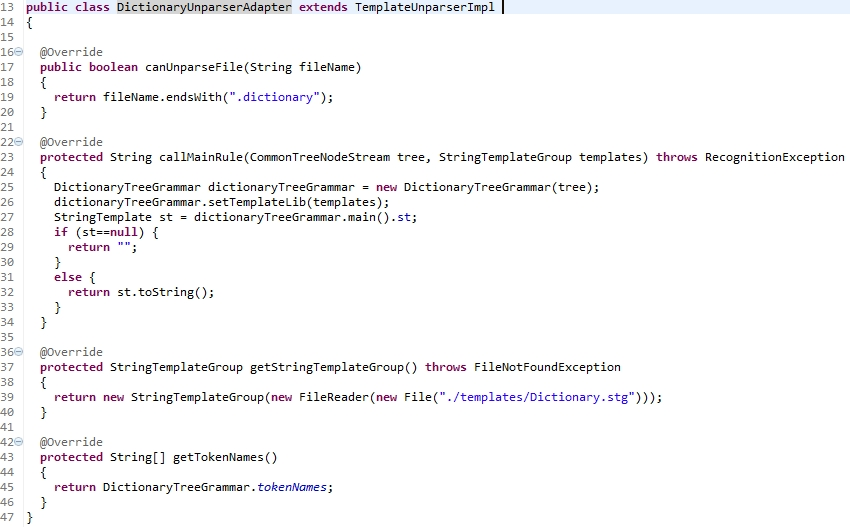
\includegraphics[width=\textwidth]{pics/moca/5MocaTreeToText/UnparserAdapter}
  \caption{Unparser Adapter} 
  \label{fig:moca-DictionaryUnparserAdapter}
\end{center}
\end{figure} 

\item[$\blacktriangleright$] Templates
  (Fig.~\ref{fig:moca-DictionaryTemplates})    
  %\usepackage{graphics} is needed for \includegraphics
\begin{figure}[!htbp]
\begin{center}
 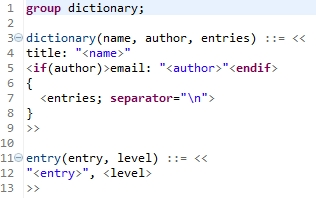
\includegraphics[width=0.6\textwidth]{pics/moca/5MocaTreeToText/DictionaryTemplates}
  \caption{Templates for the Dictionary DSL} 
  \label{fig:moca-DictionaryTemplates}
\end{center}
\end{figure} 

\item[$\blacktriangleright$] As a final step, open \texttt{MocaMain.java}
(Fig.~\ref{fig:moca-8-MocaMain}) and edit lines 41-42 as follows:
\begin{verbatim}
// Perform tree-to-text
codeAdapter.unparse("instances", out);
\end{verbatim}

%\usepackage{graphics} is needed for \includegraphics
\begin{figure}[!htbp]
\begin{center}
 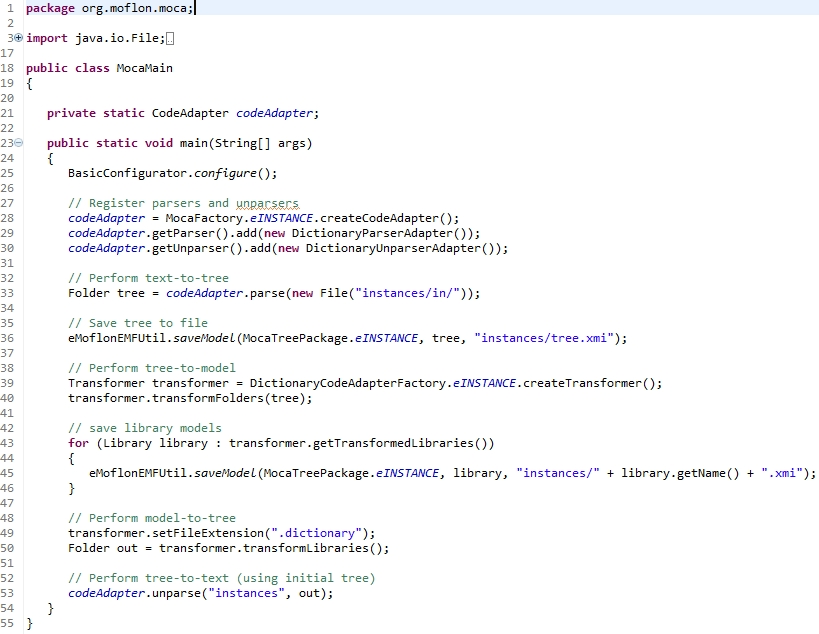
\includegraphics[width=\textwidth]{pics/moca/5MocaTreeToText/MocaMainComplete}
  \caption{Completed main method for Text-to-Model and Model-to-Text} 
  \label{fig:moca-DictionaryTemplates}
\end{center}
\end{figure}

%\usepackage{graphics} is needed for \includegraphics
\begin{figure}[!htbp]
\begin{center}
 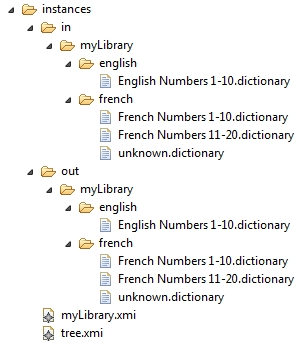
\includegraphics[width=0.6\textwidth]{pics/moca/5MocaTreeToText/InstancesAfterRoundTrip}
  \caption{Directory instances after parsing and unparsing.} 
  \label{fig:moca-DictionaryTemplates}
\end{center}
\end{figure}

\end{enumerate}